\documentclass[tikz,border=10pt]{standalone}
\usetikzlibrary{calc}

\begin{document}
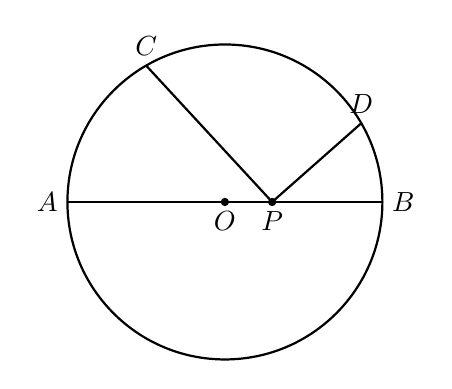
\begin{tikzpicture}
    % 定义参数
    \def\r{2} % 圆的半径
    
    % 1. 绘制圆
    \draw[thick] (0,0) circle (\r);
    
    % 2. 定义坐标
    \coordinate (O) at (0,0);
    \coordinate (A) at (-\r,0);
    \coordinate (B) at (\r,0);
    \coordinate (P) at ({0.3*\r},0); % P点位于OB之间
    \coordinate (C) at (120:\r);      % C点位于圆周，角度120度
    \coordinate (D) at (30:\r);       % D点位于圆周，角度30度
    
    % 3. 绘制元素
    % 绘制直径AB
    \draw (A) -- (B);
    % 绘制线段PC和PD
    \draw[thick] (P) -- (C);
    \draw[thick] (P) -- (D);
    
    % 4. 绘制点并标注
    \fill (O) circle (1.5pt) node[below] {$O$};
    \fill (P) circle (1.5pt) node[below] {$P$};
    
    % 放置标签
    \node[left] at (A) {$A$};
    \node[right] at (B) {$B$};
    \node[above] at (C) {$C$};
    \node[above] at (D) {$D$};

\end{tikzpicture}
\end{document}